\documentclass[11pt]{beamer}
\usetheme{PaloAlto}
\usecolortheme{spruce}
\usepackage[spanish]{babel}
\usefonttheme{professionalfonts}
\usefonttheme{serif}
\usepackage{minted}
\usepackage{fontspec}
\setmainfont{Liberation Serif}
\usepackage{amsmath}
\usepackage{amsfonts}
\usepackage{amssymb}
\usepackage{graphicx}
%Se configura minted
\definecolor{bg}{rgb}{0.95,0.95,0.95}
%\newminted{python}{fontsize=\scriptsize, 
%		   linenos,
%		   numbersep=8pt,
%		   gobble=4,
%		   frame=lines,
%		   bgcolor=bg,
%		   framesep=3mm}
\newminted{python}{fontsize=\tiny}		   
%\newminted{pycon}{bgcolor=bg, linenos=true, tabsize=4}
\newcommand{\tab}[1][1cm]{\hspace*{#1}}

\author{Nelson David Pérez Garecía\\}
\title{Introducción a Python y Obspy:\\Sesión II}
%\setbeamercovered{transparent} 
%\setbeamertemplate{navigation symbols}{} 
%\logo{} 
\institute{Servicio Geológico Colombiano} 
\date{} 
%\subject{} 
\begin{document}

\begin{frame}
\titlepage
\begin{center}
\begin{figure}

\includegraphics[scale=0.15]{Logo-SGC.jpg}
\end{figure}
\end{center}
\end{frame}

\begin{frame}
\tableofcontents
\end{frame}

\section{Introducción}
\subsection{¿Qué es Obspy?}
\begin{frame}{Obspy}
\begin{center}
\begin{figure}
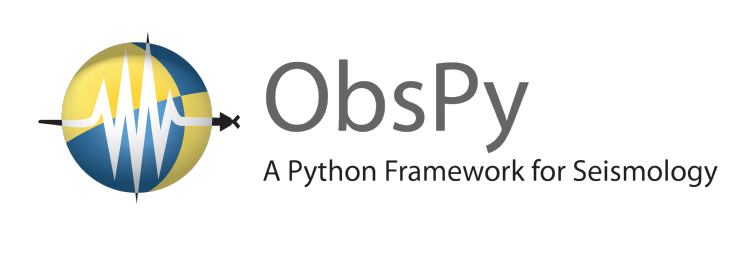
\includegraphics[scale=0.3]{obspy-logo.png}
\end{figure}
\end{center}
\end{frame}


\begin{frame}{Obspy}
\textbf{Obspy} es una libreria que permite el trabajo con datos sismológicos:
\pause
\begin{itemize}
\item Formas de onda.\\
\item Metadatos de estaciones y respuesta instrumental.\\
\item Catálogos de eventos sísmicos.\\
\end{itemize}
La última versión estable (1.0.0) se lanzó el 19 de febrero de 2016
\end{frame}

\begin{frame}{¿Cómo lo hace Obspy?}
\begin{itemize}
\item Permite lectura y escritura de datos sismológicos.
\pause
\item Permite obtener datos sismológicos de instituciones a nivel mundial y servidores a nivel local.
\pause
\item Proporciona herramientas para el manejo apropiado de metadatos.
\pause
\item Procesamiento básico de señales y análisis de datos.
\pause
\item Brinda la posibilidad de visualización.
\pause
\end{itemize}
\textbf{Obspy} utiliza como recurso otras librerias del ecosistema científico de Python: NumPy, SciPy, Matplotlib entre otros.
\end{frame}

\section{Módulos y funciones principales de Obspy}
\subsection{UTCDateTime}
\begin{frame}[fragile]{UTCDateTime}
El módulo UTCDateTime permite el manejo preciso del tiempo:
\begin{minted}{python}
>>>from obspy.core import UTCDateTime
>>>UTCDateTime("2012-09-07T12:15:00")
UTCDateTime(2012, 9, 7, 12, 15)
>>>UTCDateTime(2012, 9, 7, 12, 15, 0)
UTCDateTime(2012, 9, 7, 12, 15)
>>>UTCDateTime(1347020100.0)
UTCDateTime(2012, 9, 7, 12, 15)
\end{minted}
\end{frame}

\begin{frame}
UTCDateTime en acción...
\begin{figure}
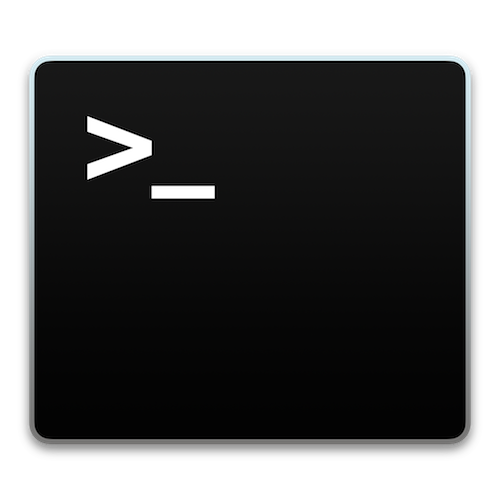
\includegraphics[scale=0.5]{terminal.png}
\end{figure}
\end{frame}

\subsection{Sismogramas}
\begin{frame}{¿Qué es un Stream?}
\begin{figure}
\begin{center}
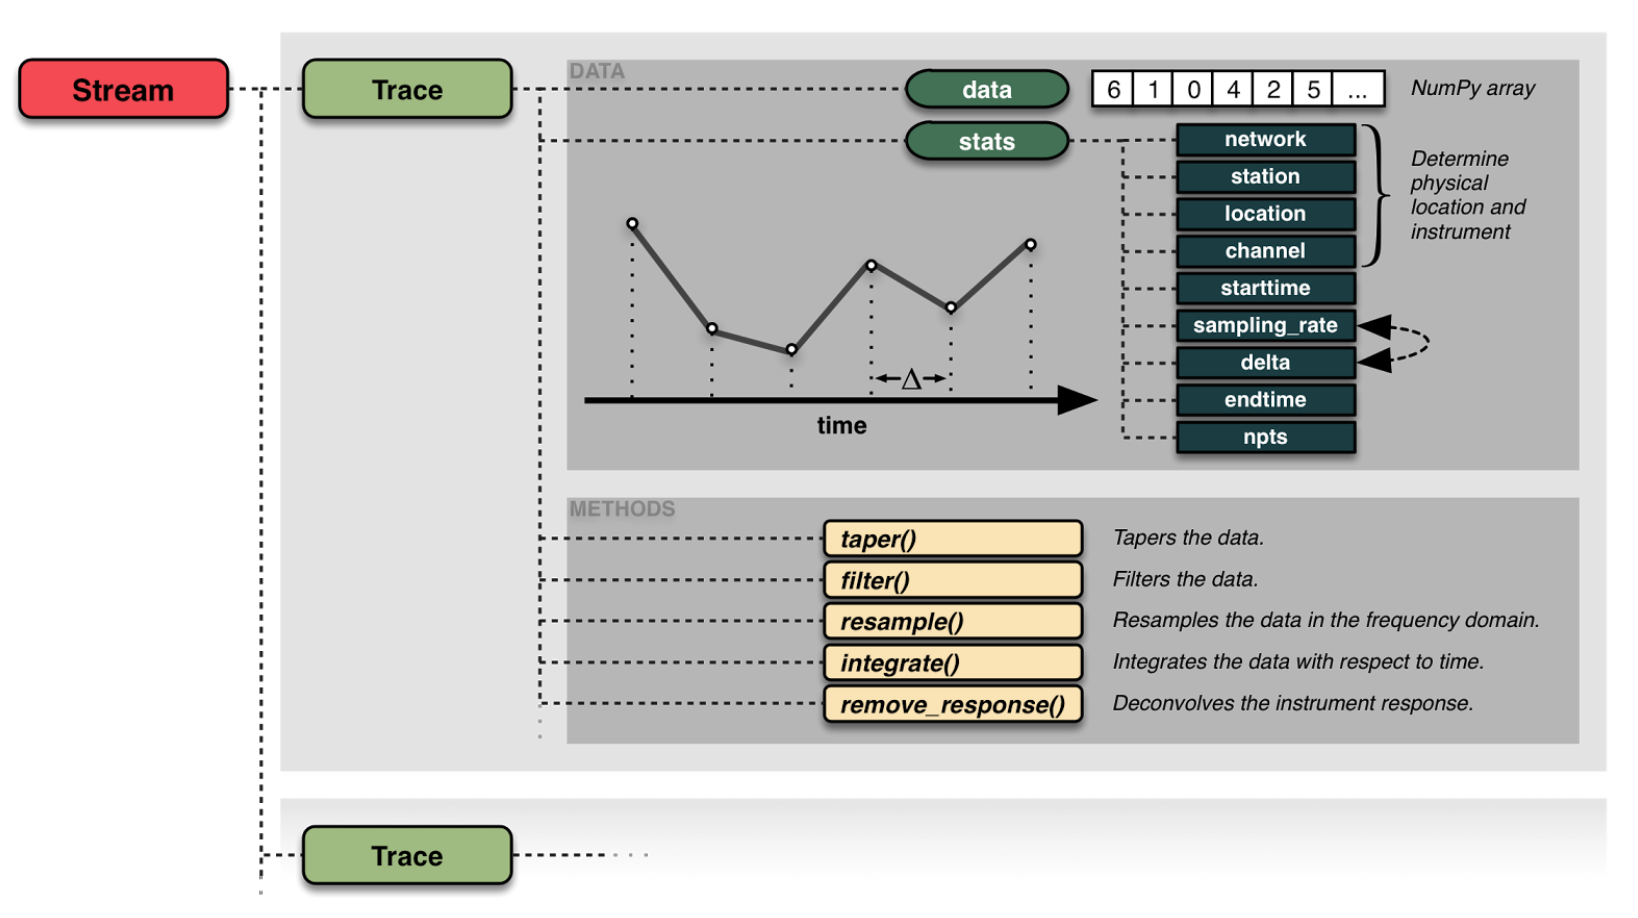
\includegraphics[scale=0.15]{stream.png}
\end{center}
\end{figure}
\end{frame}

\begin{frame}[fragile]{Lectura de sismogramas}
\begin{pythoncode}
>>>from obspy import read

>>>st = read('http://examples.obspy.org/RJOB_061005_072159.ehz.new')

>>>print(st)
1 Trace(s) in Stream:
.RJOB..Z | 2005-10-06T07:21:59.849998Z - 2005-10-06T07:24:59.844998Z | 200.0 Hz, 36000 samples

>>>len(st)
1

>>>tr = st[0]  

>>>print(tr)
.RJOB..Z | 2005-10-06T07:21:59.849998Z - 2005-10-06T07:24:59.844998Z | 200.0 Hz, 36000 sample
\end{pythoncode}
\end{frame}



\begin{frame}[fragile]{Acceso a los metadatos}
\begin{pythoncode}
>>>print(tr.stats)  
         network:
         station: RJOB
        location:
         channel: Z
       starttime: 2005-10-06T07:21:59.849998Z
         endtime: 2005-10-06T07:24:59.844998Z
   sampling_rate: 200.0
           delta: 0.005
            npts: 36000
           calib: 0.0948999971151
         _format: GSE2
            gse2: AttribDict({'instype': '      ', 'datatype': 'CM6', 
            'hang': -1.0, 'auxid': 'RJOB', 'vang': -1.0, 'calper': 1.0})

>>>tr.stats.station
'RJOB'

>>>tr.stats.gse2.datatype
'CM6
\end{pythoncode}
\end{frame}

\begin{frame}
Ejemplo con datos de la RSNC
\begin{figure}
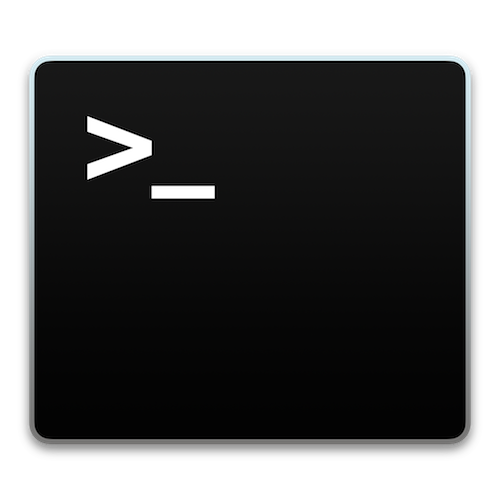
\includegraphics[scale=0.5]{terminal.png}
\end{figure}
\end{frame}

\begin{frame}[fragile]{Visualización de sismogramas}
\begin{minted}{python}
>>>st.plot()
\end{minted}
\begin{figure}
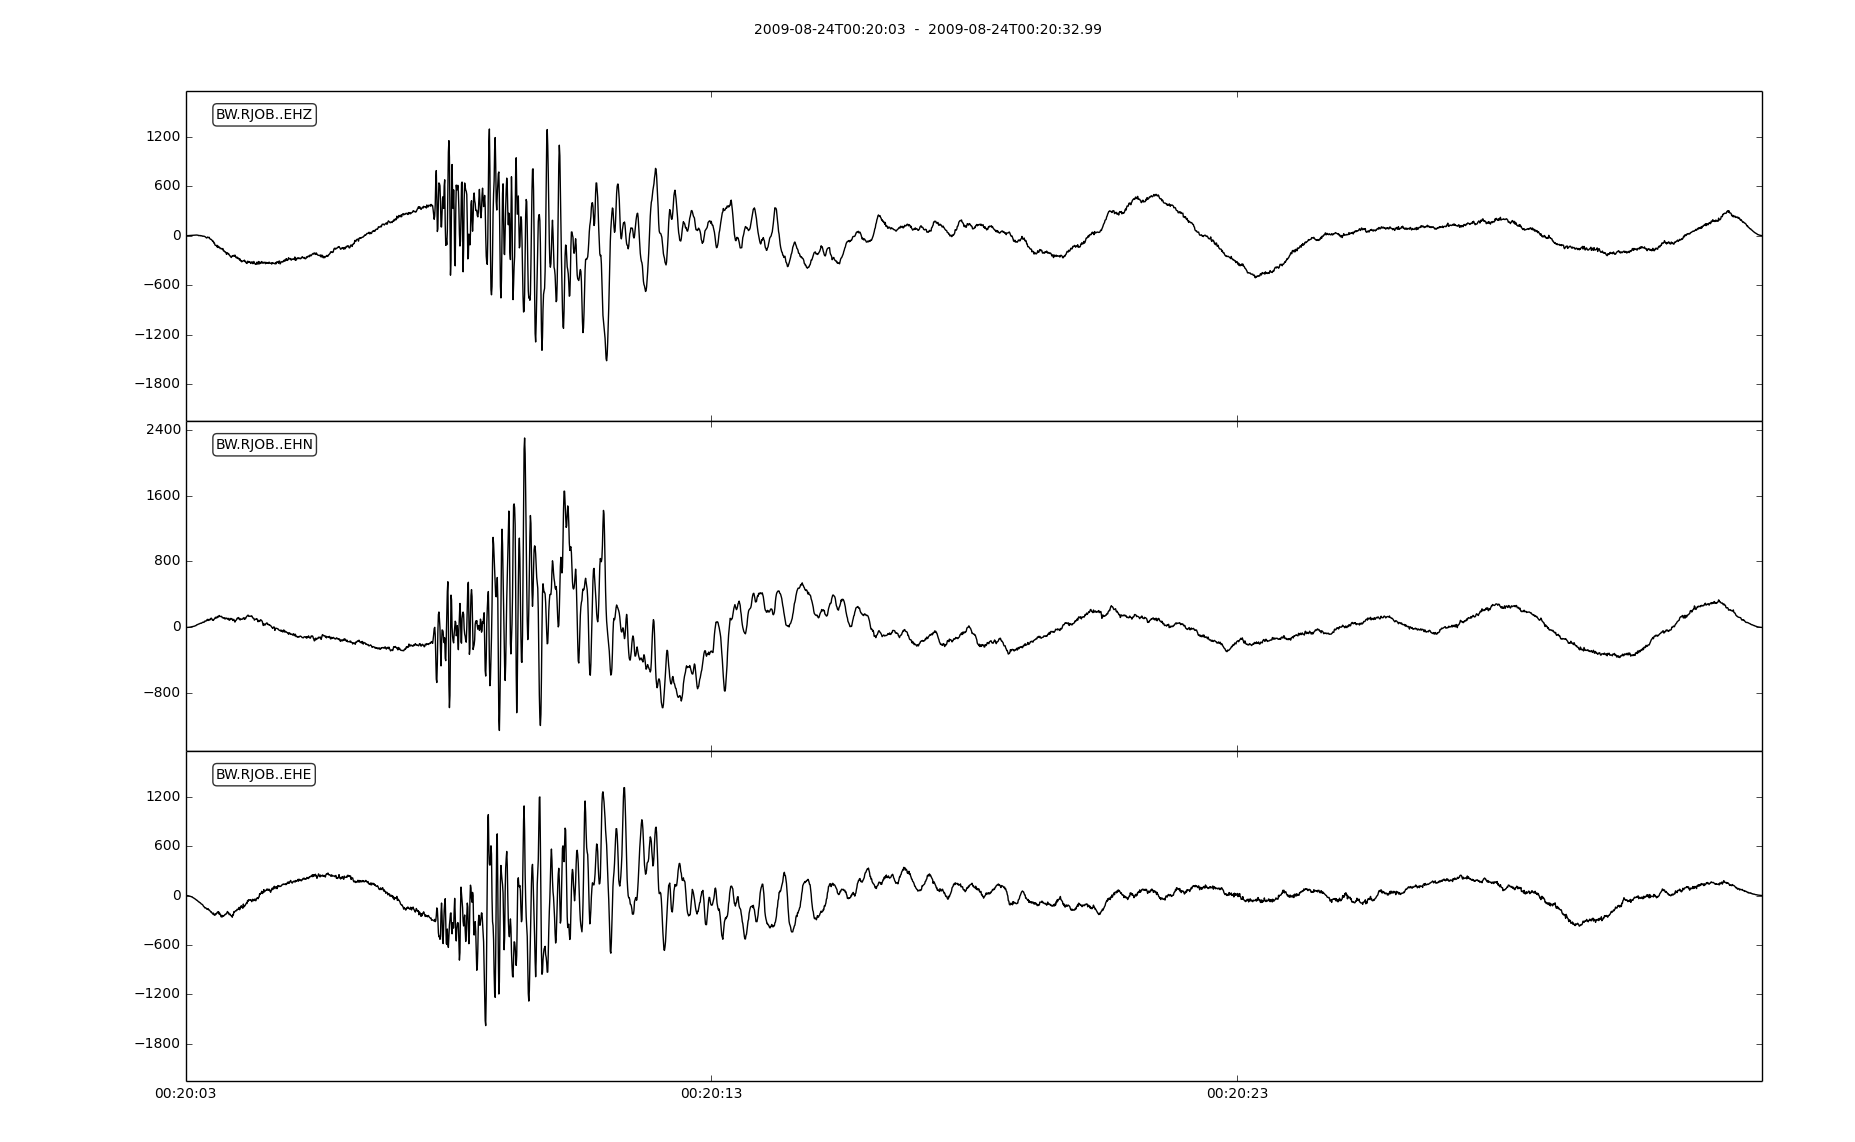
\includegraphics[scale=0.2]{traza.png}
\end{figure}
\end{frame}

\subsection{Descarga de datos sismológicos}
\begin{frame}[fragile]{Descarga de datos sismológicos}

\textbf{Obspy} permite la descarga de datos de Data Centers a nivel internacional y de servidores a nivel local mediante diferentes servicios:
\begin{itemize}
\item Servicio web FDSN.\\
\pause
\item ArcLink.\\
\pause
\item SeedLink.\\
\pause
\item IRIS.\\
\pause
\item Earthworm.\\
\end{itemize}

\end{frame}

\begin{frame}[fragile]{FDSN web service}
\begin{pythoncode}
#!/usr/bin/env python

from obspy.core import UTCDateTime
from obspy.clients.fdsn import Client
t1 = UTCDateTime(2016,03,10)
t2 = UTCDateTime(2016,03,11)
client = Client('http://10.100.100.xxx:xxxx') # se inicia el cliente FDSN

st = client.get_waveforms(starttime=t1, endtime=t2, network='CM')
\end{pythoncode}
\end{frame}

\subsection{Inventarios y Catálogos}

\begin{frame}[fragile]{Inventarios}
\begin{minted}{python}
>>>import obspy
>>>inv = obspy.read_inventory('inventory.xml')
>>>inv.plot('local')
\end{minted}
\begin{figure}
\begin{center}
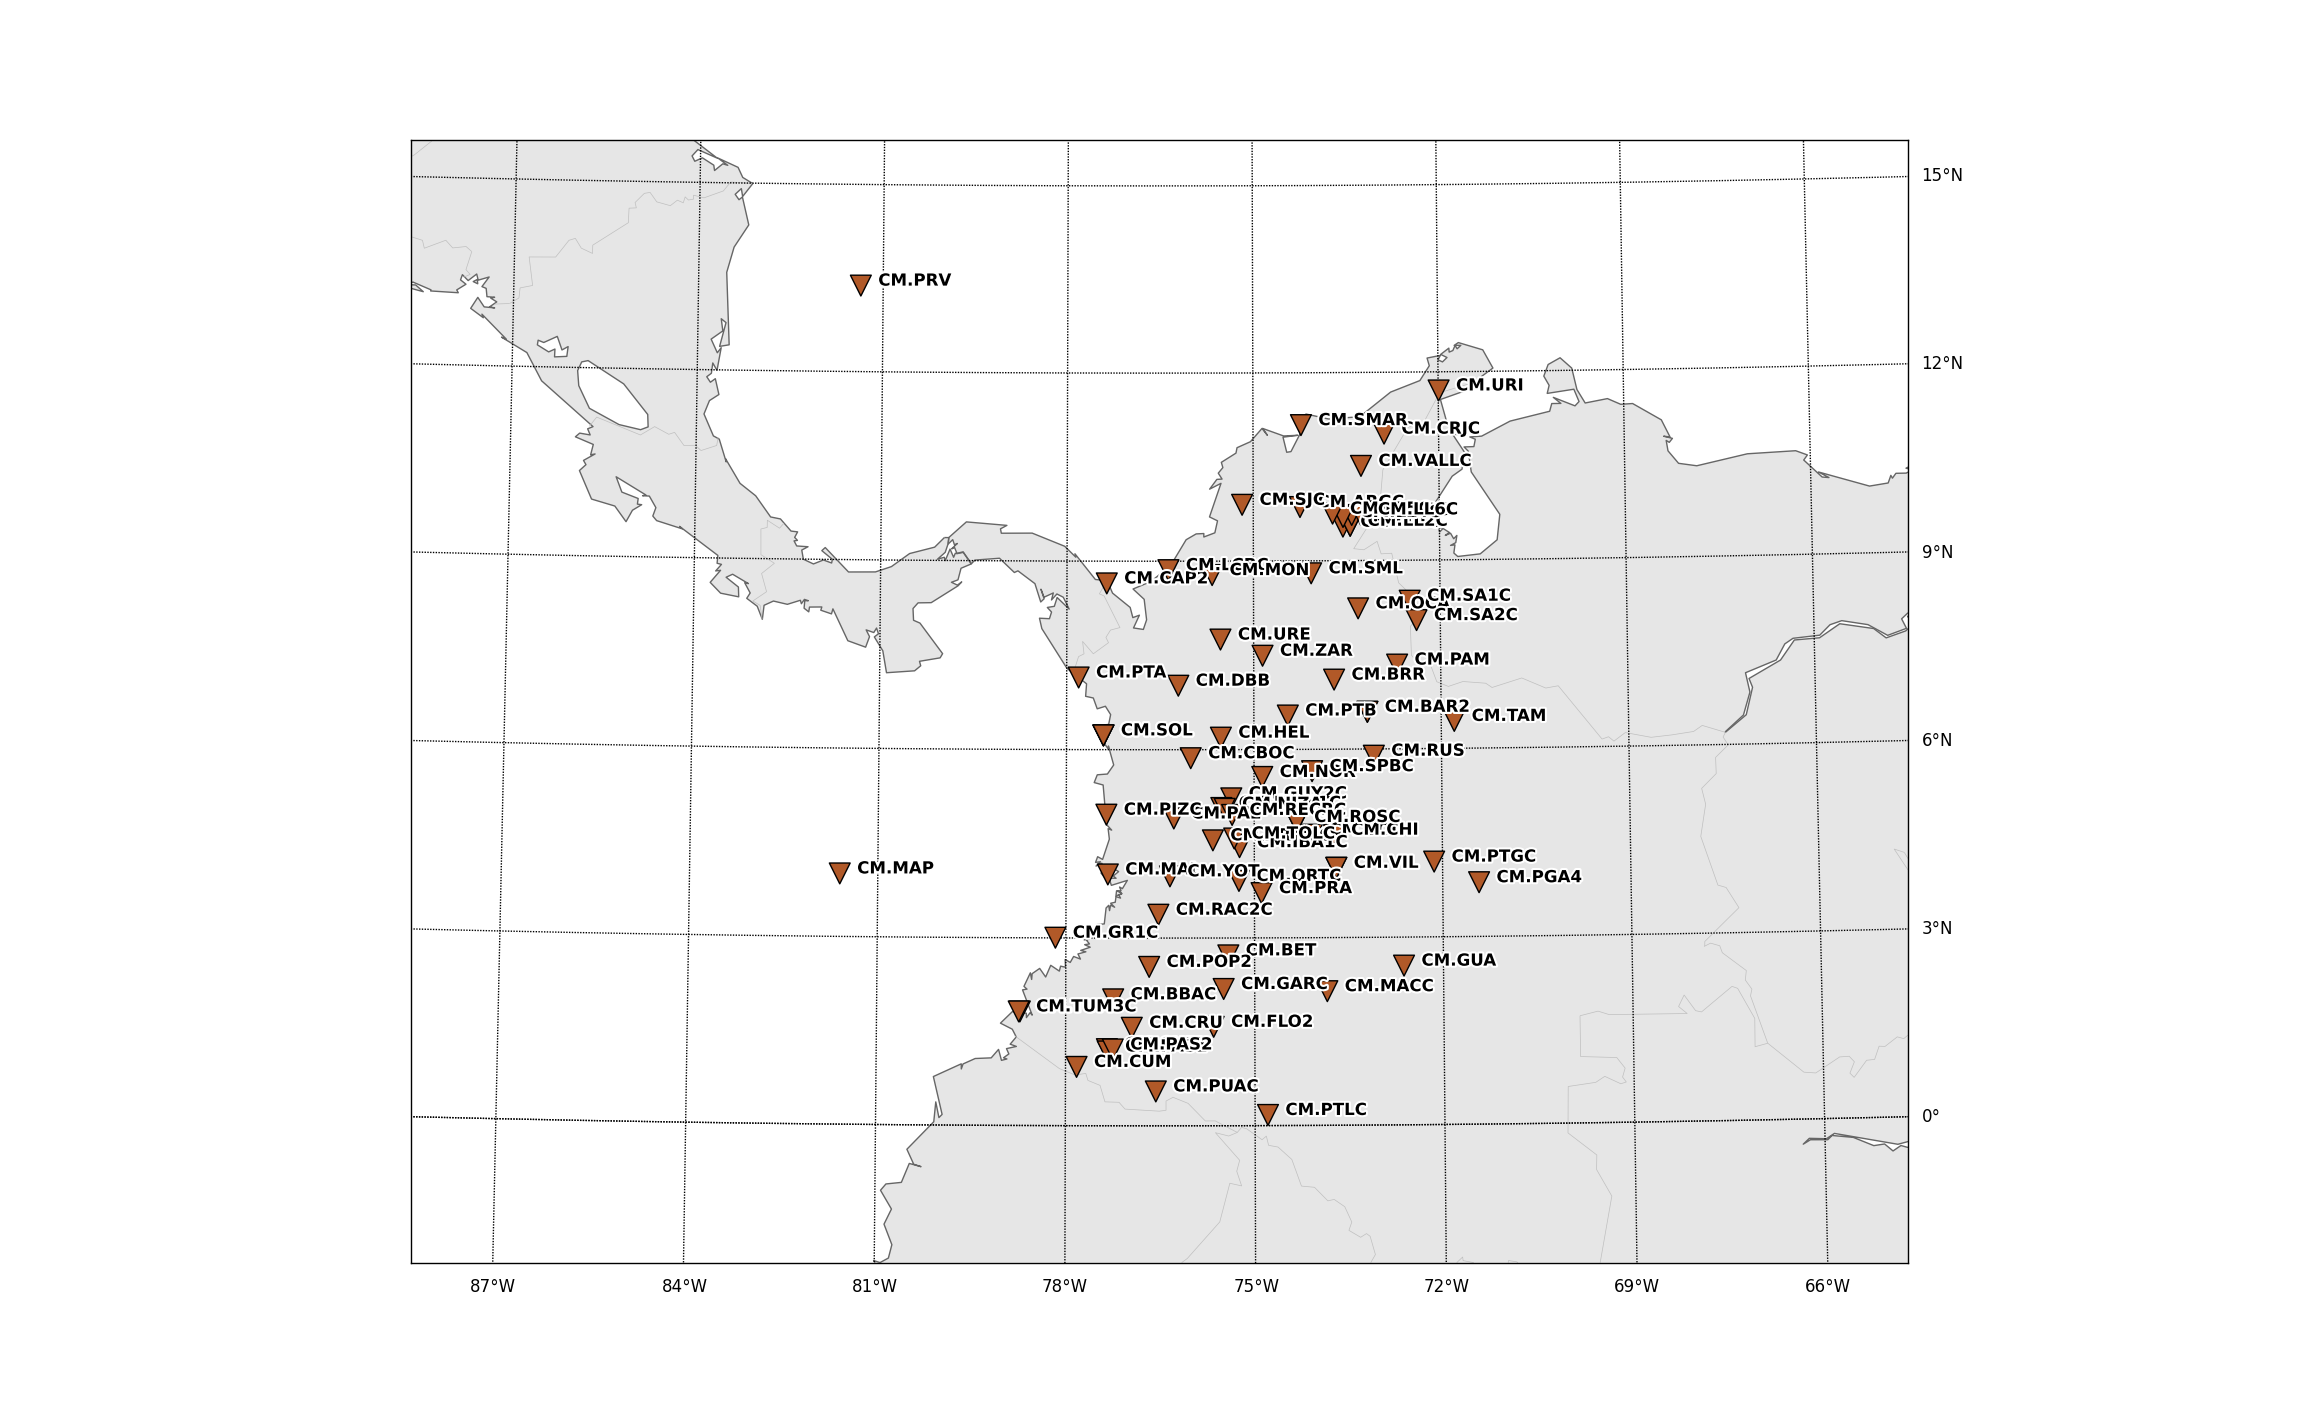
\includegraphics[scale=0.15]{inventario.png}
\end{center}
\end{figure}
\end{frame}

\begin{frame}{Inventarios}
\begin{figure}
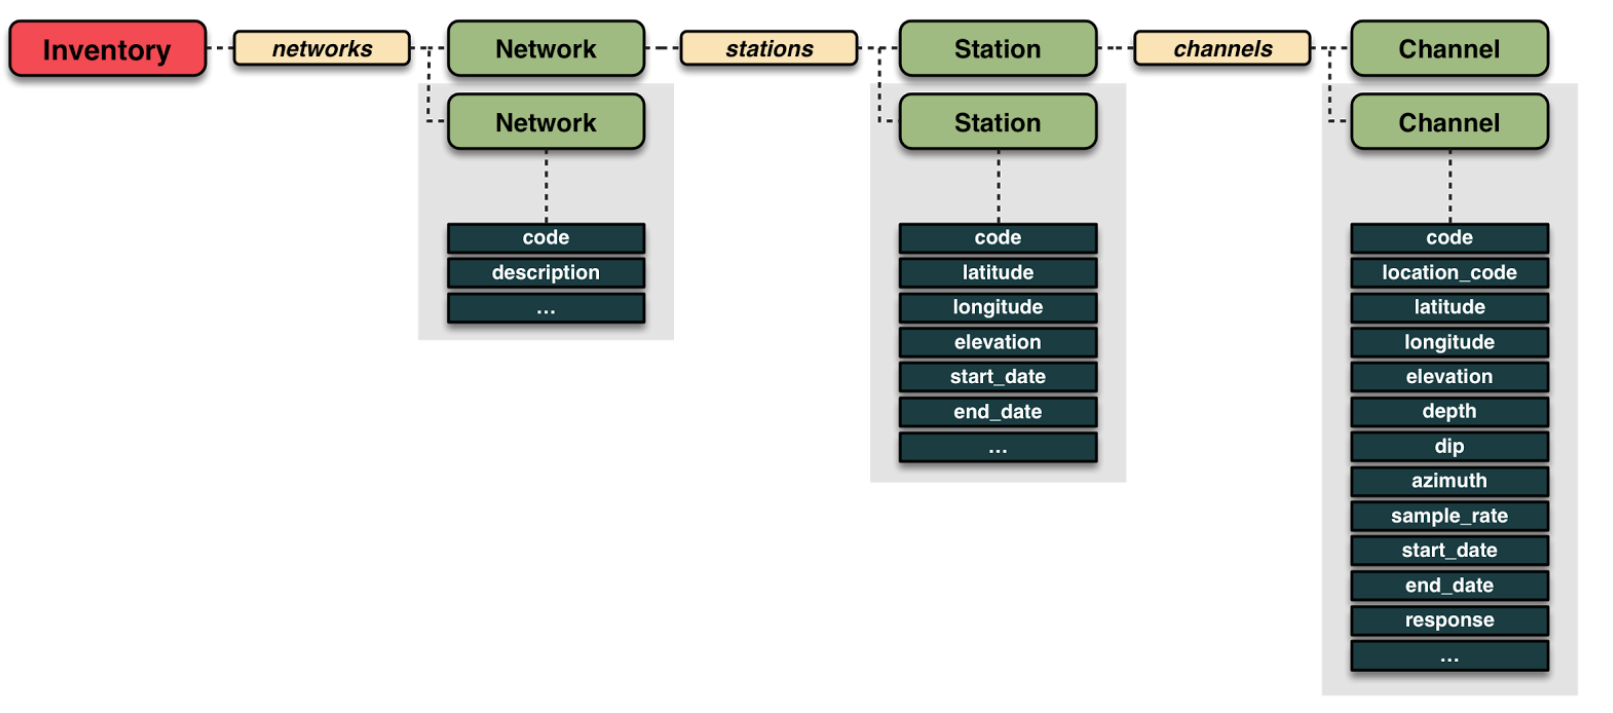
\includegraphics[scale=0.15]{inv.png}
\end{figure}
\end{frame}

\begin{frame}[fragile]{Catálogos}
\begin{minted}{python}
>>>import obspy
>>>cat = obspy.read_events('catalog.xml')
>>>cat.plot('local')
\end{minted}
\begin{figure}
\begin{center}
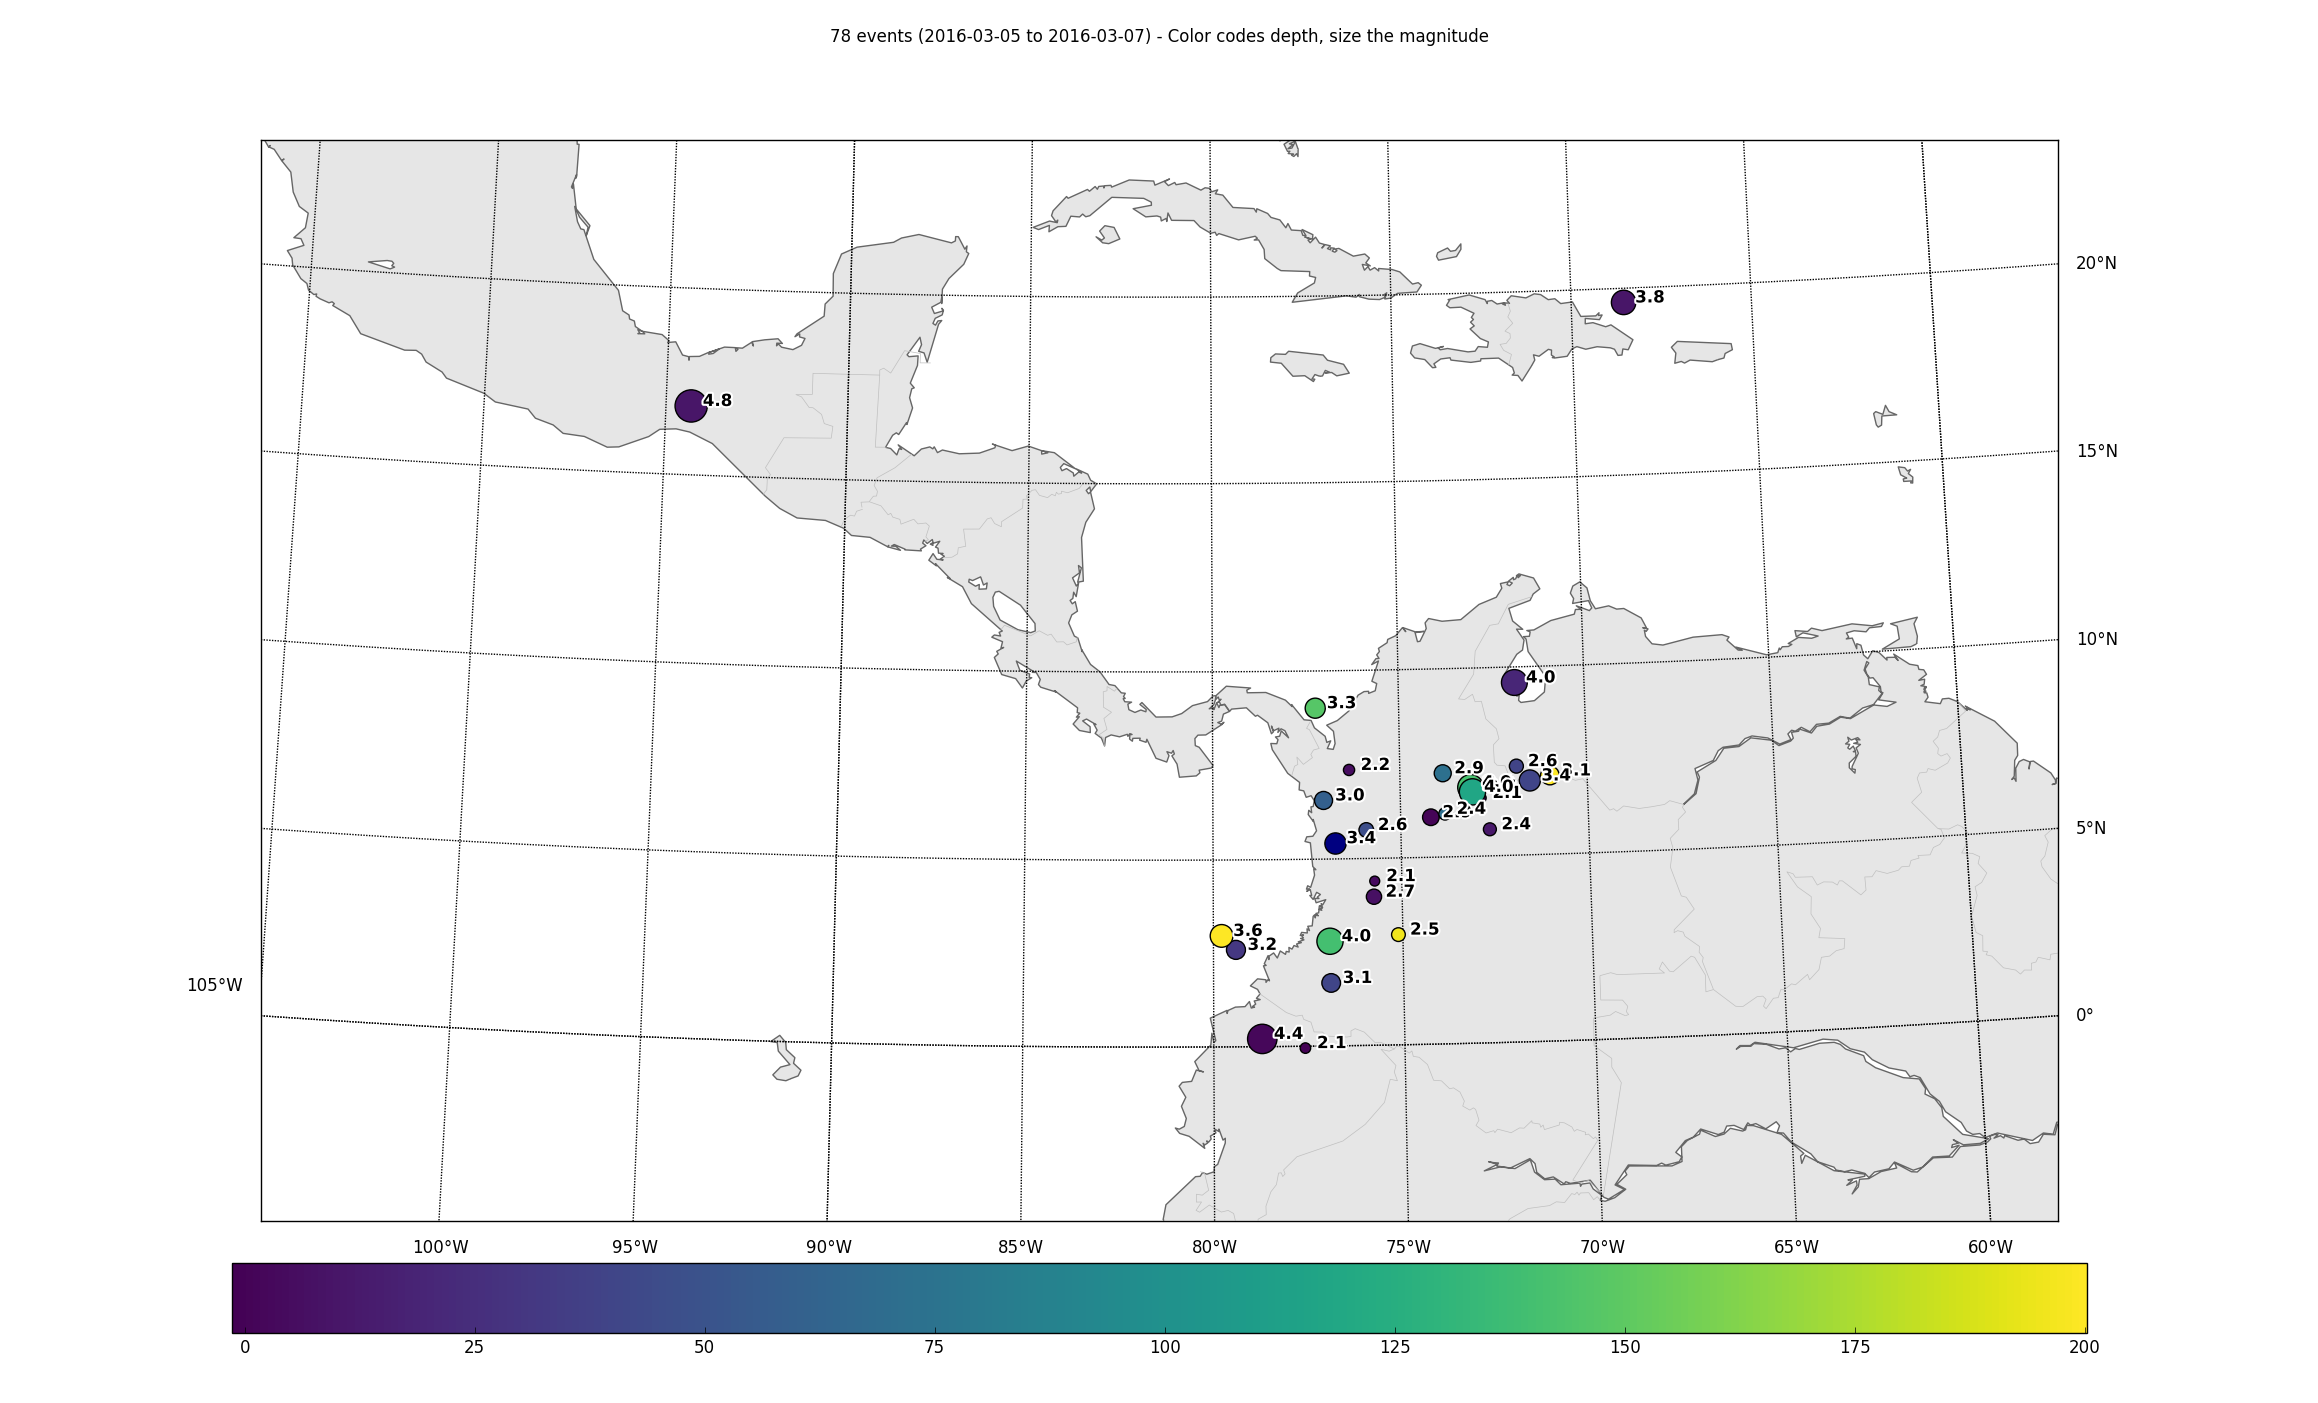
\includegraphics[scale=0.15]{cat.png}
\end{center}
\end{figure}
\end{frame}

\begin{frame}{Catálogos}
\begin{figure}
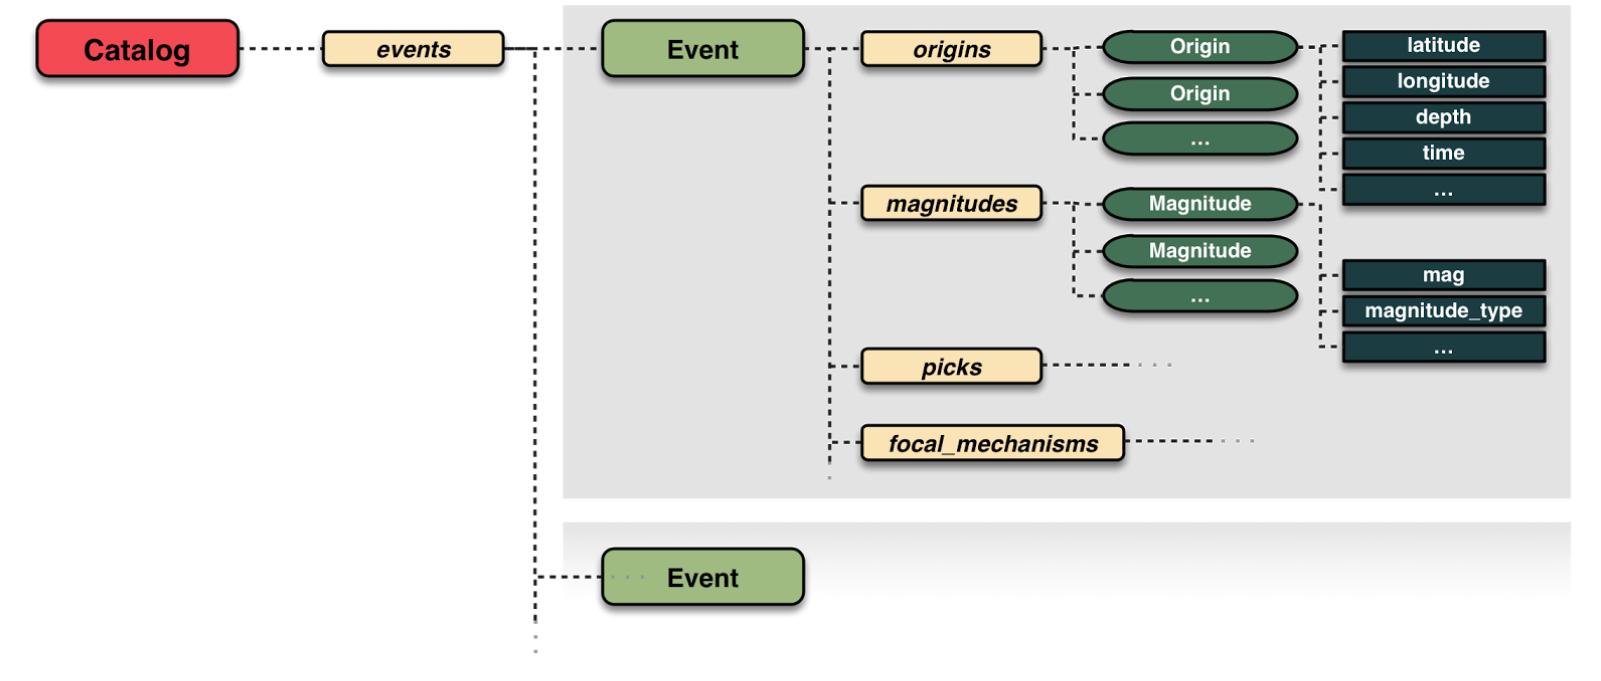
\includegraphics[scale=0.15]{catalog.png}
\end{figure}
\end{frame}

\section{Aplicaciones}
\subsection{Respuesta Instrumental}
\begin{frame}[fragile]{Respuesta Instrumental}
Se puede visualizar la respuesta instrumental de un sismómetro junto a la forma de onda corregida:
\begin{minted}{python}
from obspy import read, read_inventory

st = read("/path/to/IU_ULN_00_LH1_2015-07-18T02.mseed")
tr = st[0]
inv = read_inventory("/path/to/IU_ULN_00_LH1.xml")
pre_filt = [0.001, 0.005, 10, 20]
tr.remove_response(inventory=inv, pre_filt=pre_filt, output="DISP",
                   water_level=60, plot=True)
\end{minted}
\end{frame}

\begin{frame}{Respuesta Instrumental}
\begin{figure}
\begin{center}
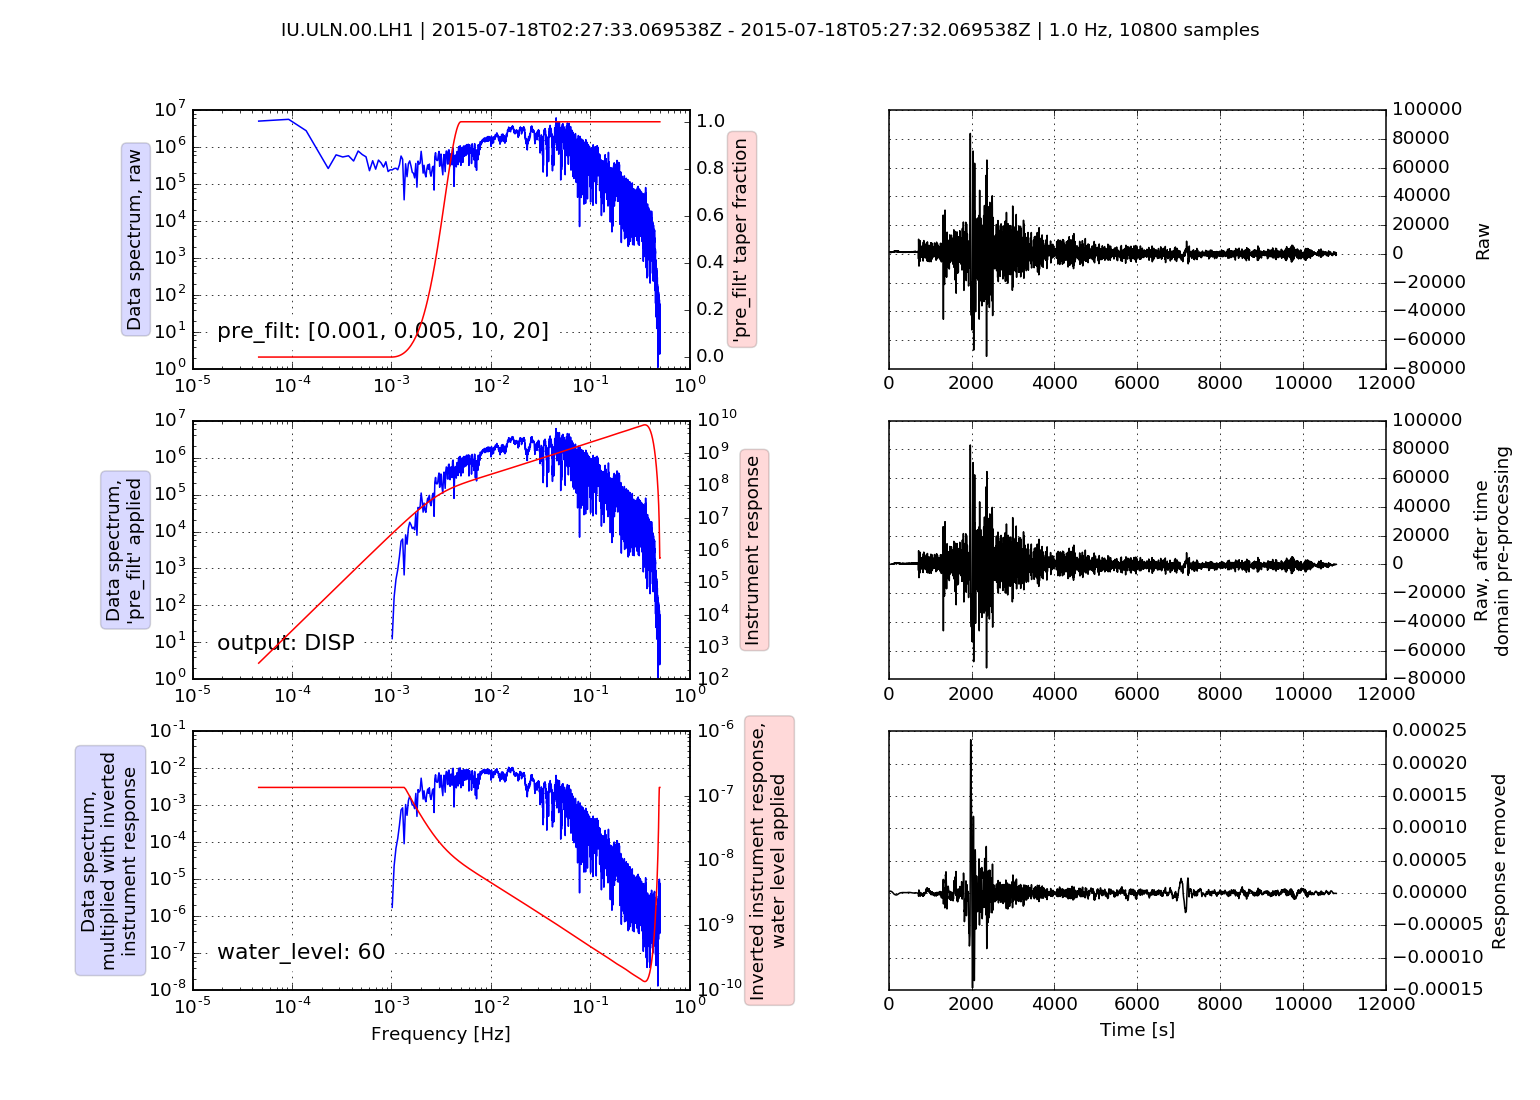
\includegraphics[scale=0.2]{respuesta.png}
\end{center}
\end{figure}
\end{frame}
\end{document}